%%%%%%%%%%%%%%%%%%%%%%%%%%%%%%%%%%%
%This is the LaTeX ARTICLE template for RSC journals
%Copyright The Royal Society of Chemistry 2014
%%%%%%%%%%%%%%%%%%%%%%%%%%%%%%%%%%%

\documentclass[twoside,twocolumn,9pt]{article}
\usepackage{extsizes}
\usepackage[super,sort&compress,comma]{natbib} 
\usepackage[version=3]{mhchem}
\usepackage[left=1.5cm, right=1.5cm, top=1.785cm, bottom=2.0cm]{geometry}
\usepackage{balance}
\usepackage{packages/widetext}
\usepackage{times,mathptmx}
\usepackage{sectsty}
\usepackage{graphicx} 
\usepackage{lastpage}
\usepackage[format=plain,justification=raggedright,singlelinecheck=false,font={stretch=1.125,small,sf},labelfont=bf,labelsep=space]{caption}
\usepackage{float}
\usepackage{fancyhdr}
\usepackage{hyperref}
\usepackage{lscape}
\usepackage{bibunits}
\usepackage{fnpos}
\usepackage[english]{babel}
\usepackage{array}
\usepackage{amsmath}
\usepackage{amssymb}
\usepackage{easySymbols}
\usepackage{supplemental}
\usepackage{droidsans}
\usepackage{charter}
\usepackage[T1]{fontenc}
\usepackage[usenames,dvipsnames]{xcolor}
\usepackage{setspace}
\usepackage[compact]{titlesec}
%%%Please don't disable any packages in the preamble, as this may cause the template to display incorrectly.%%%


\usepackage{epstopdf}%This line makes .eps figures into .pdf - please comment out if not required.

\definecolor{cream}{RGB}{222,217,201}

\begin{document}

\pagestyle{fancy}
\thispagestyle{plain}
\fancypagestyle{plain}{

%%%HEADER%%%
\fancyhead[C]{
\includegraphics[width=18.5cm]{head_foot/header_bar}}
\fancyhead[L]{\hspace{0cm}\vspace{1.5cm}
\includegraphics[height=30pt]{head_foot/journal_name}}
\fancyhead[R]{\hspace{0cm}\vspace{1.7cm}
\includegraphics[height=55pt]{head_foot/RSC_LOGO_CMYK}}
\renewcommand{\headrulewidth}{0pt}
}
%%%END OF HEADER%%%

%%%PAGE SETUP - Please do not change any commands within this section%%%
\makeFNbottom
\makeatletter
\renewcommand\LARGE{\@setfontsize\LARGE{15pt}{17}}
\renewcommand\Large{\@setfontsize\Large{12pt}{14}}
\renewcommand\large{\@setfontsize\large{10pt}{12}}
\renewcommand\footnotesize{\@setfontsize\footnotesize{7pt}{10}}
\makeatother

\renewcommand{\thefootnote}{\fnsymbol{footnote}}
\renewcommand\footnoterule{\vspace*{1pt}% 
\color{cream}\hrule width 3.5in height 0.4pt \color{black}\vspace*{5pt}} 
\setcounter{secnumdepth}{5}

\makeatletter 
\renewcommand\@biblabel[1]{#1}            
\renewcommand\@makefntext[1]% 
{\noindent\makebox[0pt][r]{\@thefnmark\,}#1}
\makeatother 
\renewcommand{\figurename}{\small{Fig.}~}
\sectionfont{\sffamily\Large}
\subsectionfont{\normalsize}
\subsubsectionfont{\bf}
\setstretch{1.125} %In particular, please do not alter this line.
\setlength{\skip\footins}{0.8cm}
\setlength{\footnotesep}{0.25cm}
\setlength{\jot}{10pt}
\titlespacing*{\section}{0pt}{4pt}{4pt}
\titlespacing*{\subsection}{0pt}{15pt}{1pt}
%%%END OF PAGE SETUP%%%

%%%FOOTER%%%
\fancyfoot{}
\fancyfoot[LO,RE]{\vspace{-7.1pt}
\includegraphics[height=9pt]{head_foot/LF}}
\fancyfoot[CO]{\vspace{-7.1pt}\hspace{13.2cm}
\includegraphics{head_foot/RF}}
\fancyfoot[CE]{\vspace{-7.2pt}\hspace{-14.2cm}
\includegraphics{head_foot/RF}}
\fancyfoot[RO]{\footnotesize{\sffamily{1--\pageref{LastPage} ~\textbar  \hspace{2pt}\thepage}}}
\fancyfoot[LE]{\footnotesize{\sffamily{\thepage~\textbar\hspace{3.45cm} 1--\pageref{LastPage}}}}
\fancyhead{}
\renewcommand{\headrulewidth}{0pt} 
\renewcommand{\footrulewidth}{0pt}
\setlength{\arrayrulewidth}{1pt}
\setlength{\columnsep}{6.5mm}
\setlength\bibsep{1pt}
%%%END OF FOOTER%%%

%%%FIGURE SETUP - please do not change any commands within this section%%%
\makeatletter 
\newlength{\figrulesep} 
\setlength{\figrulesep}{0.5\textfloatsep} 

\newcommand{\topfigrule}{\vspace*{-1pt}% 
\noindent{\color{cream}\rule[-\figrulesep]{\columnwidth}{1.5pt}} }

\newcommand{\botfigrule}{\vspace*{-2pt}% 
\noindent{\color{cream}\rule[\figrulesep]{\columnwidth}{1.5pt}} }

\newcommand{\dblfigrule}{\vspace*{-1pt}% 
\noindent{\color{cream}\rule[-\figrulesep]{\textwidth}{1.5pt}} }

\makeatother
%%%END OF FIGURE SETUP%%%

%%%TITLE, AUTHORS AND ABSTRACT%%%
\twocolumn[
  \begin{@twocolumnfalse}
\vspace{3cm}
\sffamily
\begin{tabular}{m{4.5cm} p{13.5cm} }


\includegraphics{head_foot/DOI} & \noindent\LARGE{\textbf{GeneSPIDER - Gene regulatory network inference benchmarking with controlled network and data properties$^\dag$}} \\%Article title goes here instead of the text "This is the title"
\vspace{0.3cm} & \vspace{0.3cm} \\

 & \noindent\large{Andreas Tj{\"a}rnberg\textit{$^{a, b,c,\ast}$}}, {Daniel C. Morgan\textit{$^{a,b,\ast}$}}, {Matthew Studham\textit{$^{a,b}$}}, Torbj{\"o}rn E. M. Nordling\textit{$^{a,d,{\ast}{\ast},{\ddag}}$} and {Erik L.L. Sonnhammer\textit{$^{a,b,{\ast}{\ast},{\ddag}}$}} \\%Author names go here instead of "Full name", etc.


\includegraphics{head_foot/dates} & \noindent\normalsize{% \textcolor{red}{
A key question in network inference, that has not been properly answered, is what accuracy can be expected for a given biological dataset and inference method. We present \gs--a Matlab package for tuning, running, and evaluating inference algorithms that allows independent control of network and data properties to enable data-driven benchmarking. \gs is uniquely suited to address this question by first extracting salient properties from the experimental data and then generating simulated networks and data that closely match these properties.%}
It enables data-driven algorithm selection,  estimation of inference accuracy from biological data, and a more multifaceted benchmarking. 
Included are generic pipelines for the design of perturbation experiments, bootstrapping, analysis of linear dependence, sample selection, scaling of SNR, and performance evaluation.
With \gs we aim to move the goal of network inference benchmarks from simple performance measurement to a deeper understanding of how the accuracy of an algorithm is determined by different combinations of network and data properties.
} \\

\end{tabular}

 \end{@twocolumnfalse} \vspace{0.6cm}

  ]
%%%END OF TITLE, AUTHORS AND ABSTRACT%%%

%%%FONT SETUP - please do not change any commands within this section
\renewcommand*\rmdefault{bch}\normalfont\upshape
\rmfamily
\section*{}
\vspace{-1cm}

%%%FOOTNOTES%%%

\footnotetext{\textit{$^{a}$Stockholm Bioinformatics Center, Science for Life Laboratory, Sweden}}
\footnotetext{\textit{$^{b}$Department of Biochemistry and Biophysics, Stockholm University, Sweden. }}
\footnotetext{\textit{$^{c}$Department of Physics, Chemistry and Biology, Link\"oping University, Sweden. }}
% \footnotetext{\textit{$^{c}$Department of Immunology, Genetics and Pathology, Uppsala University, Rudbeck laboratory, 75185, Uppsala, Sweden.}}
\footnotetext{\textit{$^{d}$Department of Mechanical Engineering, National Cheng Kung University, No. 1 University Road, 70101, Tainan, Taiwan.}}

% \footnotetext{\textit{$^{x}$These authors contributed equally to this work}}
\footnotetext{\textit{$^{\ast}$These authors contributed equally to this work}}
\footnotetext{\textit{$^{\ast\ast}$These authors contributed equally to this work}}

%Please use \dag to cite the ESI in the main text of the article.
%If you article does not have ESI please remove the the \dag symbol from the title and the footnotetext below.
\footnotetext{{\dag}Electronic Supplementary Information (ESI) available: %[\textbf{Availability and Implementation: 
Source code freely available for download at 
\url{https://bitbucket.org/sonnhammergrni/genespider}, implemented in Matlab.}

\footnotetext{\textit{${\ddag}$Contact: 
\url{torbjorn.nordling@nordlinglab.org}, \url{erik.sonnhammer@scilifelab.se}}

\textbf{Supplementary information:} online-only supplementary data available at the journal's web site.]. See DOI: 10.1039/b000000x/}
%additional addresses can be cited as above using the lower-case letters, c, d, e... If all authors are from the same address, no letter is required

%\footnotetext{\ddag~Additional footnotes to the title and authors can be included \emph{e.g.}\ `Present address:' or `These authors contributed equally to this work' as above using the symbols: \ddag, \textsection, and \P. Please place the appropriate symbol next to the author's name and include a \texttt{\textbackslash footnotetext} entry in the the correct place in the list.}


%%%END OF FOOTNOTES%%%

%%%MAIN TEXT%%%%
\begin{bibunit}
\section{Introduction}

The goal of gene regulatory network (GRN) inference is to understand
how genes influence each other in terms of their expression, i.e. to
unravel the transcriptional regulatory influences \cite{Hecker2009}.
A primary objective in network inference is to obtain a network where each link corresponds to a true regulatory interaction in the biological system, i.e. to avoid false positives.
A secondary objective is that each real link becomes inferred, i.e. to avoid false negatives.
The quality of the inferred network model, that is, the number of false positives and negatives, depends both on the inference method and the data.
Here we focus on dynamic models of regulatory networks and algorithms that are designed to take these effects into account.

Benchmarks are a common method to objectively compare performance of different network inference algorithms. Famous challenges, such as the DREAM challenge \citep{Marbach2012}, are designed around data sets from multiple "gold standard" biological systems where the known links or the network's main properties are assumed true.

In practice, artificial networks and data from simulated experiments are commonly used due in part to the current lack of a "true" network of gene regulation for any biological system, as well as the temporal and monetary ease of generating data \insilico. In particular, the properties of the networks and data are easier to adapt to the specific needs of a project.
Simulations often meet biological experiments half way by incorporating knowledge derived from \invivo data to create realistic networks and \insilico datasets \citep{Bansal2007,Hache2009,Narendra2011,Penfold2011}.
For example, a substantial number of transcriptional regulatory interactions are known for \Coli and \Yeast, and can be used when deciding the structure of the artificial network model \citep{Salgado2013,Teixeira2013}.
However, it is important to distinguish between
(i) networks and data that are intended to mimic real biology as closely as possible, and
(ii) networks and data that are intended to be approximations, only capturing certain properties of their counterparts.

\begin{figure*}
\centering
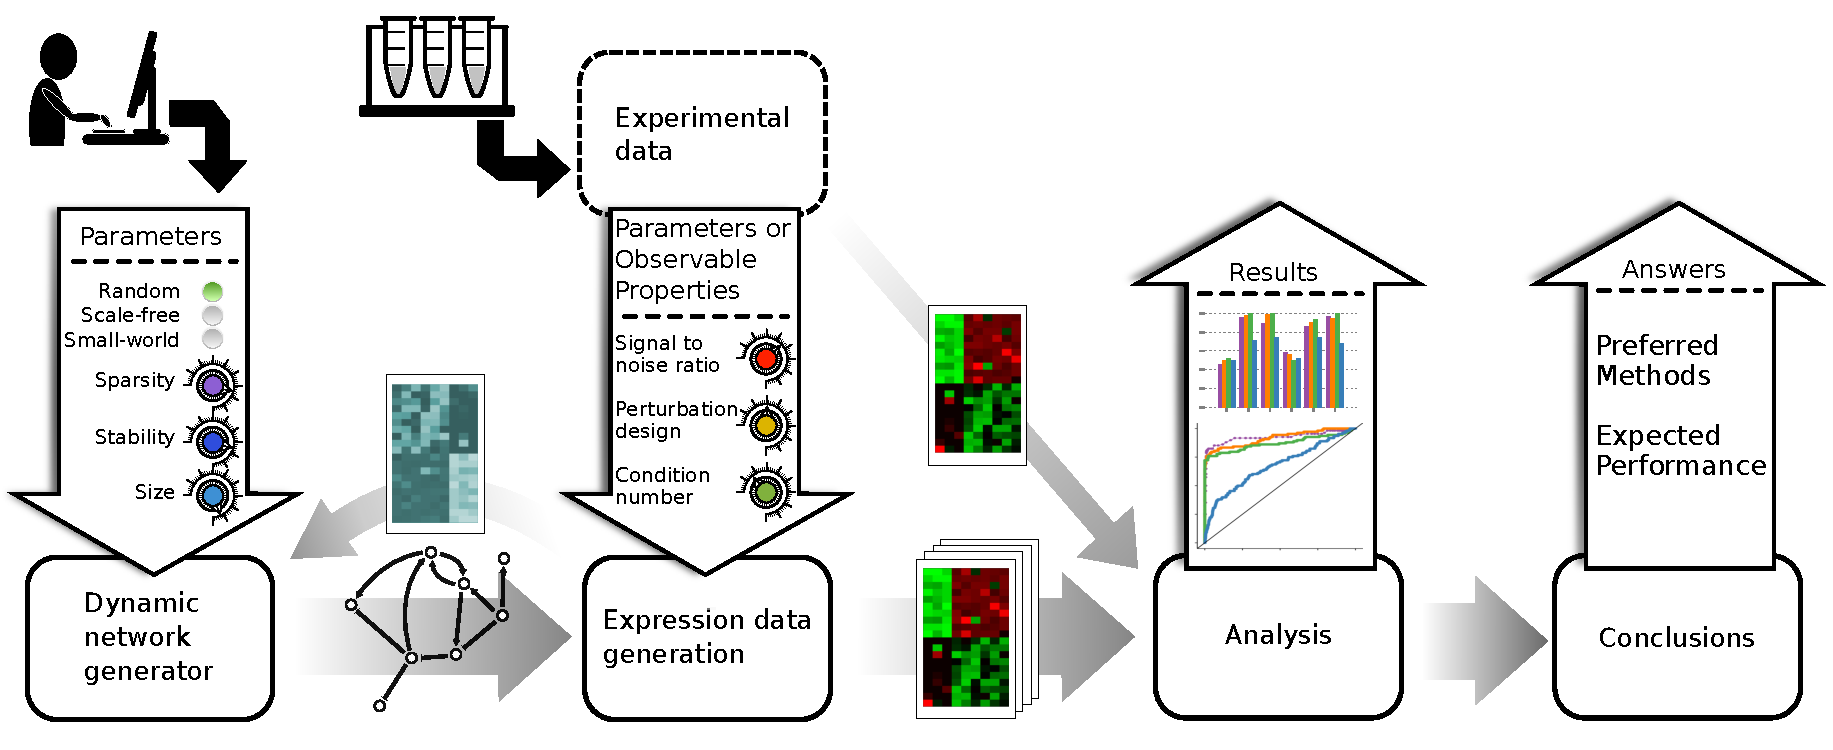
\includegraphics[width=0.9\textwidth]{img/pipeline.pdf}
\captionsetup{width=0.9\textwidth}
\caption{Schematic workflow of network and data generation followed by analysis in \gs. (i) Import or generate networks with a range of properties; stabilize and modify the interampatteness degree. (ii) Generate expression data with specific SNR, perturbation design, and condition number. (iii) Analyze GRN inference benchmark results in relation to the network and data properties. (iv) Draw conclusions about which methods to use under what conditions. The figure also shows an alternative path where \gs extracts properties from experimental data in order to generate simulated networks and data.  Such a benchmark provides information about the expected accuracy for a given real dataset.}
\label{fig:benchmark-pipeline}
\end{figure*}

The network construction process usually involves modelling networks as a system of ordinary differential equations (ODEs), with e.g. linear \citep{Bansal2007}, or nonlinear \citep{VandenBulcke2006,Schaffter2011} models.
The perturbation, \ie system input, used in the experimental design is typically a single gene knockdown/knockout, or a system wide perturbation, \ie a perturbation that randomly alters multiple genes at a time.

To streamline the creation of new benchmarks of network inference methods several packages have been published to facilitate the creation a benchmark data sets and networks \citep{VandenBulcke2006,Hache2009b,DiCamillo2009,Schaffter2011}.
A common feature of these benchmarking packages is the focus on network structure as the main feature controllable by the user.
\emph{\syntren} \citep{VandenBulcke2006} utilizes selected dynamic structures and sub-networks from biological systems, \coli and \yeast.
\emph{\netsim} \citep{DiCamillo2009} takes a different approach by generating dynamical models, incorporating structurally random network motifs, which they dub modular topology models.
\emph{\genge} \citep{Hache2009b} uses a nonlinear model similar to \syntren and allows for the generation of networks with specific network motifs.
All the above methods utilize some form of non-linear dynamics to produce gene expressions from the network structure. 

The GRN inference community has organized around challenges, such as the DREAM
challenge, to benchmark network inference methods by applying them to the same data and comparing their performance \citep{Marbach2012}.
The package \emph{\gnw} \citep{Schaffter2011} expands upon ideas similar to those of the \emph{\syntren} and \emph{\genge} packages and is used to create datasets for these challenges.
\emph{\gnw} enables the user to choose among a variety of \insilico standard perturbation designs when generating networks and time-series data, as well as to define the number of nodes and in-degree.
Its nonlinear dynamical model and simulated data are based on several types of omics data in order to mimic a real biological system.

Publicly available gene expression datasets typically suffer from few data points compared to the high number of genes and possible interactions, large measurement uncertainty both in the perturbations and responses, \ie poor signal to noise ratio (SNR), and redundant nearly collinear variables, \ie ill-conditioned data matrices \citep{Nordling2013phdthesis}.
Considering this, previously published benchmark packages support surprisingly few perturbation design alternatives and data properties.
Noise is typically added to the input and/or output as a percentage of the magnitude of the applied perturbation or measured signal, rather than the SNR. Due to the ill-conditioning, the former does not typically allow for control of the later.
% \textcolor{red}{
In a similar ambition as Kurtz et al.\cite{SPIEC-EASI2015}, we seek to control certain aspects of data generation.%}
However, no previously published package makes it clear to what extent the specific model, or the perturbation design, effects the data generated or the inference being made.
None of the previously published packages facilitate this analysis. Nor do they facilitate control of observable data properties, such as the SNR and ill-conditioning, which as we have demonstrated should be used to guide the algorithm selection \citep{Tjarnberg2014}.

The DREAM challenge, for example, does not define observable properties that could guide a choice of inference method or give an estimate of how informative the dataset is. Instead it focuses on network properties and motifs when trying to evaluate to what extent a specific inference approach is useful.
While this might reveal hard to infer motifs and network structures, it becomes meaningless when faced with a dataset since the motifs can not be observed a priori.
Furthermore, the perturbation design is not connected to the network properties, thus equal perturbation design could give arbitrarily "good" or "bad" data given a specific network model.
While an algorithm may generally perform well, it might act to the contrary faced with a specific set of data properties.

% \textcolor{red}{
A more recent benchmarking package, \netbenchmark \citep{Bellot2015}, aims to evaluate inference methods by bundling datasets from \emph{Rogers simulator}\cite{rogers2005bayesian}, \emph{\syntren}  and \emph{\gnw}, and benchmarking across several existing inference algorithms in a unified workbench. However, the fundamental issues of the methods aggregated are neither solved nor addressed, simply evaluated in the same way.%}
Benchmarks should provide guidance on both (i) which inference method to use for a particular dataset, and (ii) which errors to expect in the inferred network. Benchmarking should be a data driven procedure.

Here we present \gs, a benchmarking suite designed specifically to deal with the issues presented above.
\gs focuses on key properties influencing inference performance \cite{Tjarnberg2014}, allowing the user to "tune" certain parameters in the context of the core functionality expected from a benchmarking suite. 
In the generation of the dynamical network model, \gs focuses on stability\cite{Zavlanos2011} and interampatteness \cite{Nordling2009}.
By interampatteness we mean the ratio between the system's ability to amplify and attenuate different signals, which for a linear system corresponds to the condition number of the network matrix. This is strongly correlated with the difficulty of inferring the correct network, as attenuated signals typically are hidden in the noise and essentially determines the accuracy of the inferred network, since network inference is an inverse problem\cite{Nordling2013phdthesis}.

The observed signal is determined by the applied perturbation and the attenuation of it by the system. The strength of the perturbations could and should be scaled to counteract the intrinsic attenuation of signals.
The condition number of the dataset has been shown to serve as a proxy for the interampatteness in the context of known perturbations\cite{Nordling2013phdthesis,Tjarnberg2014}. 
The benefit here is that the condition number of the dataset can be observed and hence provide information on how difficult it is to infer a specific network from the available data.

The noise estimate in the direction of the data's smallest variation is expected to have the greatest impact on the data quality, as in any inverse problem.
Therefore we provide variation estimates and apply noise scaled towards the principle directions of variance in the data (by default the smallest).
Since the variation in the data can be distributed very differently among the directions from one dataset to the next, this is necessary to correctly see what effect a certain level of noise can have on the data.
This makes it possible to have two observable properties, signal to noise ratio and the condition number of the data, as tune-able parameters not previously incorporated into benchmarking pipelines, yet informative for property-dependent error analysis and confidence estimation. 
This informs the user how informative the data set is and what performance should be expected from different methods, as shown previously \cite{Tjarnberg2013,Tjarnberg2014}.

\gs improves upon existing packages by providing a data driven approach to benchmarking focused on independently controlling properties of network and data. This is essential for establishing the relation between properties and inference accuracy. One of the most important questions in network inference is what accuracy can be expected for a given real dataset. \gs is able to address this question by extracting salient properties from experimental data and then generate simulated networks and data that closely match these properties (See Figure \ref{fig:benchmark-pipeline}).
In this article we demonstrate the workflow of \gs Figure \ref{fig:benchmark-pipeline}, with code examples given in the Supplementary Information, in order to lower the initial usage threshold, focusing on generating approximations with tuned properties and avoiding unnecessary complexity in order to gain insight.


\section{Methods and GeneSPIDER capabilities}
\label{sec:methods}
The functions in the following sections cover the five typical phases in benchmarking of inference methods based on \insilico experiments: 
Generation of network models (phase A), design of perturbation experiments (phase B), simulations of the designed experiments on the generated systems (phase C), inference of network models from the simulated datasets using the methods of interest (phase D), and analysis of the performance of the methods (phase E).

\subsection{Model formalism and notation}
\label{sec:model_formalism}

A linear dynamical system described by ordinary differential equations (ODEs),
\begin{equation}
  \begin{array}{r c l}
    \frac{d}{dt} \check{x}_i(t) &=& \sum_{j=1}^N \check{a}_{ij} \check{x}_j(t) + p_i(t) - f_i(t)\\
    y_i(t) &=& \check{x}_i(t) + e_i(t),
  \end{array}
  \label{eq:linearsys}
\end{equation}

\noindent
is used to approximate the local behaviour of a biological system in the current version of \gs.
This approximation is commonly used to describe GRNs, see \eg \citet{Yuan2011,Gardner2003}.
In GRNs the state vector \(\check{\bx}(t)=[\check{x}_1(t),\check{x}_2(t),\ldots,\check{x}_N(t)]^T\) represents actual mRNA expression changes relative to the initial state of the system in \(\breve{N}\) genes.
The vector \(\bp(t)=[p_1(t),p_2(t),\ldots,p_N(t)]^T\) represents the applied perturbation, which, in general, is corrupted by the noise \(\bbf(t)\).
The perturbations could be \eg gene siRNA knock-downs or gene over-expressions using a plasmid with an extra copy of the gene.
The response vector \(\by(t)=[y_1(t),y_2(t),\ldots,y_N(t)]^T\) represents the measured expression changes, which is the ``true" expression corrupted by the noise \(\be(t)\).
Our network is the interaction matrix with parameters \(\check{a}_{ij}\), which represent the influence of an expression change of gene \(j\) on gene \(i\).
A positive value of \(\check{a}_{ij}\) represents an activation, while a negative value represents an inhibition.
The value of the \(\check{a}_{ij}\) parameter gives the relative strength of the interaction.
Here \(\; \check{} \;\) is used to mark ``true" variables that are not corrupted by noise or measurement errors.


\subsection{Network generation}
\label{sec:network_generation}

Network generation (phase A) is done in four steps: (i) generation of a network graph with desired topology, (ii) assignment of random weights to the links, (iii) stabilization of the system, and (iv) tuning of the IAA degree of the system corresponding to the network.

\gs includes three algorithms for directed and undirected network topology generation (step i): random, scale-free, and small-world; auto-regulation/degradation self-loops are supported for directed networks.
The desired number of links is set by providing a sparsity parameter to the algorithm. The sparsity is defined as \(s=L/N^2\), where \(L\) is the number of links in the network and \(N^2\) the number of possible links in a directed graph.
The algorithm generating random graphs, where each link has the same probability \(p_l\) to exist, is based upon the assumption that every graph, \(G(N,L)\), is equally probable \citep{Erdos1961}.
The algorithm generating scale-free graphs \citep{Barabasi1999}, where each node added to the network is attached to previous nodes with a probability \(p_l\) proportional to the number of edges each of the previous nodes has, is based upon the preferential attachment principle \citep{Reka-Barabasi2002}.

This algorithm produces a network with bidirectional links only. 
However, directed biological networks rarely have bidirectional links, so we at random eliminate one of the links in each symmetric link pair with probability \(p_{\text{remove}}\), implying that we keep both with probability \(1-p_{\text{remove}}\). When eliminating a link we eliminated the outgoing link $a_{ji}$ with probability \(p_{\text{outgoing}}\).

The algorithm generating small-world graphs \citep{Watts1998}, where nodes are serially connected with the \(l\) closest neighbours in a ring lattice, is based on the implementation suggested by \citet{Prettejohn2011}. Each node is then considered to randomly be disconnected from a neighbour and reconnected to another node in the ring lattice.
Graphs that are partly scale-free can be generated by seeding the preferential attachment algorithm with \eg a small-world network so that a small-world-scale-free (SW-SF) network is generated.

After the topological layout, a weight is assigned to each link present by assigning weights drawn from a iid normal distribution with mean zero and standard deviation one (step ii).
This is done in order to convert the graph into a dynamical system. The weight \(\check{a}_{ij}\) of each link that is present determines the effect that node \(j\) has on node \(i\).

% \textcolor{red}{
Since a stable system guarantees that all quantities remain finite, a stable network model is typically desired. The weighted network may therefore need to be stabilized (step iii) and have its condition number tuned, \ie tuning of the interampatteness (IAA) degree \citep{Nordling2009}. IAA is a generic property of biochemical networks, akin to the data property collinearity.%}
When assigning random weights to each link there is no guarantee that the resulting system is stable. Stability is guaranteed if all eigenvalues of the interaction matrix are negative. 
Data generation for benchmarking of inference algorithms should be restricted to stable systems, because, while the local linearisation of a globally stable nonlinear system can be unstable \citep{Khalil1996}, it is not possible to infer an unstable linear system in practice; even the smallest amount of process noise will move the system away from the unstable steady-state.
Note that every isolated system must be globally stable, or risk some state variable (mRNA abundance) becoming infinite and violating mass-conservation laws.
We assure stability by employing a method that forces all eigenvalues of our interaction matrix to be negative\citep{Zavlanos2011}, enabling the creation of a stable linear dynamic system from most unstable network graphs.
However, this does not work for all graphs because the algorithm is based on making the diagonal dominating and negative, whereupon addition of a few links typically solves the problem.
% \textcolor{red}{
The algorithm forces the eigenvalues to be negative by incorporation of a convex optimization protocol\citep{grant2008cvx}. While  convexity guarantees that the algorithm for each initial network returns only one final network, two different initial networks may yield the same final network.
Desired network properties can be arrived upon by iterating over the substantially reduced space of stable linear dynamical systems.%}

The IAA degree tuning (step iv) is enabled by the user defining limits on the eigenvalues of the network in the convex optimization.
This sets an upper bound on the inverse condition number, which can be infeasible or arbitrarily conservative.
In practice, one therefore needs to generate a network ensemble with different random topological weights and select those of condition number (IAA degree) within the desired interval. Note that links are removed if their strength falls below a user defined threshold.
This ensures that we keep link strengths within a reasonable range to avoid trivial links as well as possible numerical issues when working with the network in subsequent steps.
However, this can result in a slight deviation from the desired sparsity.

\subsection{Data generation}
\label{sec:data_generation}


The purpose of the experiment design (phase B) is to generate a perturbation matrix \(\mP\), containing either a sequence of perturbations in a time-series experiment or a sequence of steady-state experiments. 
Only a small number of genes should be perturbed in each perturbation, so that it may be practically implemented \invivo or \invitro given current technical limitations.
Publicly available real gene expression datasets have either been generated by perturbing one gene at a time (single gene perturbation), two genes at a time (double gene perturbations), or by a system perturbation, such as a change in environmental factors or introduction of a drug, which is thought to affect several genes at once but typically is quantitatively unknown.
These perturbations are trivial to generate in \matlab using \eg the function for generation of diagonal random matrices \texttt{diag(randn(N,M))} or sparse random matrices \texttt{sprandn(N,M)}.

We also provide a method to generate a pseudo-optimal perturbation design that counteracts intrinsic signal attenuation based on an inversion of the ``true" system. 
Small elements in the designed perturbation matrix \(\mP\) are removed to make it sparse, while keeping the condition number of the response matrix \(\kappa(\mY)\)  close to 1.
This implies that the response matrix will be close to an identity matrix, with equal signal strength in \(N\) linearly independent directions.
Note that while this method cannot be used for biological experiments (because the ``true" system is unknown), it can be used to generate informative datasets for benchmarking.

The experiments are simulated (phase C) either by calculating the steady-state response, as in equation (\ref{eq:Linearmap}), or the time-series response, as in equation (\ref{eq:linearsys}).
The system dynamics are simulated with a time step \(t = \tau_N/10\), where \(\tau_N\) is the smallest time constant of the system given by the eigenvalues of the network matrix.
We typically first simulate noise-free measurements and then add noise drawn from the desired distribution, typically a standardized normal distribution with zero mean and variance one.
This enables us to tune the SNR by scaling the noise matrix, which for normally distributed noise corresponds to scaling of the standard deviation, such that the desired SNR is obtained. 

\label{sec:data-analysis}

\subsection{GRN inference methods}
\label{sec:inference-methods}
A core piece of any inference pipeline is the inference method itself, which takes data and algorithm parameters as input and yields one or several network estimates as output (phase D). In \gs we have created wrappers with a common entry format for a number of published and in-house inference methods to simplify their use, see Table \ref{tab:gs-methods}. Wrappers make it easy to incorporate future inference algorithms and provide the same benchmark capabilities in our standardised environment.

We here introduce a modified version of the Robust Network Inference algorithm (RNI)\citep{Nordling2013phdthesis} by applying a range of cut-offs to the confidence scores, and call this version RNI cut-off (RNICO). This way different network estimates ranging from empty to full are obtained by gradually lowering the confidence cut-off independent of how informative the data is, while native RNI for uninformative data produce an empty network.  
The significance level \(\alpha=0.01\) was used in RNICO to scale Nordling's confidence score such that every link with a value above one exists in the true network for 99 out of every 100 links fulfilling this criterion. 

\subsection{Evaluation of inferred networks}
\label{sec:evaluation_of_networks}

Measures of network similarity are needed to assess the performance of any given inference method (phase E), and we have decided to implement many such measures to accommodate researchers' preference.
\gs currently provides a function for comparison of networks that includes 18 system measures, 3 signed topological measures, 1 correlation measure, 12 graph measures, and 9 directed graph measures, see section \ref{sec:compare-models}.
The \gs toolbox includes many standard measures of performance, including MCC and AUROC, with which to compare available inference pipelines and tune such for specific dataset properties.


\subsection{Quantification of network and system properties}
\label{sec:quantification_network_properties}

To investigate if a relation exists between a network property and \eg the performance of an inference algorithm, the network property first needs to be objectively quantified and a measure of it implemented.
\gs contains functionality for the calculation of basic graph properties, such as number of nodes and links, basic topology measures reported in \citet{Prettejohn2011} such as the clustering coefficient, the degree distribution, the average path length, and advanced measures such as the number of strong components. We calculate these measures for each network structure based on the network type, either directed or undirected. We have also implemented functions for calculation of system properties, such as the time constant and IAA degree.


\subsection{Quantification of data properties}
\label{sec:quantification_data_properties}

For the expression data we have tried to quantify the informativeness and difficulty to infer the correct network in terms of signal to noise ratio, similarity between experiments, and the condition number.
\gs contains several different SNR calculations; see definitions in section \ref{sec:SNR}. The condition number is calculated with the \matlab function \texttt{cond}.
\section{A case study using the benchmark suite}
\label{sec:results}
To demonstrate the application of \gs we generated a benchmark suite of 200 networks and 600 expression datasets that includes networks of four different topologies with varied IAA degrees and sizes. Based on these we simulated data each with three SNR variants, and analyzed the performance of four GRN inference methods in relation to the properties of the networks and expression data. 
The four methods tested in this benchmark are ARACNe \citep{margolin2006aracne}, least squares cut-off (LSCO) \citep{Tjarnberg2013}, RNICO, and the Glmnet implementation of \lasso \citep{Tibshirani1996,Friedman2010}.
Figure \ref{fig:benchmark-pipeline}, gives an overview of the \gs workflow and some parameters of networks and data that are possible to vary.

\subsection{Network generation}
\label{sec:network-generation}
We generated 10 networks of sizes \(N\in \{10,50,100\}\) for each of the four classes: random, small-world, scale-free and small-world-scale-free, and for each of two IAA levels, \(\kappa \in \{low,high\}\). In total 200 networks were generated. Scale-free and small-world-scale-free are missing for \(N=10\) because this is to small for scale-free like properties to be relevant. The small-world networks only have high IAA degree because of limitations in the IAA adjustment method compounded by the fact that cascades, which are present in small-world networks due to the initial ring lattice, in general increases the IAA degree \citep{Nordling2009}.
The two IAA degree levels were: IAA degree of 9$N$ to 11$N$ (high) and IAA degree of 0.5$N$ to $N$ (low).
We scaled the IAA degree with the network size because the condition number of a random matrix with normally distributed entries tends to grow with the matrix size.
The IAA degree of each network is shown in Figure \ref{fig:iaa}.

IAA can be difficult to tune for certain network structures and sparsity levels, so we
allowed some flexibility relative to the specified sparsity.
In particular, networks with a low IAA degree are difficult to find for very sparse networks, since they tend to contain cascade and feedback loops that in general increase the IAA degree. We therefore implemented a larger sparsity coefficient for these sparse networks, \ie the addition of one or two links to the network, with secondary link addition if the algorithm had trouble stabilizing the network at the desired IAA degree.
Performance analysis of the network inference methods was carried out on multiple 10-gene random networks.

The sparsity coefficient was set for each network generation method, scaled by the size of the network to maintain a relatively low mean degree per node, so all networks can be considered truly sparse.
The sparsity ranges of the different network topology classes and sizes in this benchmark are shown in Table \ref{tab:sparsity}.
The degree distributions for each network topology class and size are shown in Figure \ref{fig:out-degree}.

\begin{table}[htb]
\caption{\label{tab:sparsity}
Properties of networks in this benchmark. Self-loops are included. SW-SF stands for small-world and scale-free.}
\centering
\begin{tabular}{|l|r|r|r|r|}
\hline
Network class & N & Sparsity & Links & Avg degree\\
\hline
random & 10 & 0.25 & 25 & 2.5\\
 & 50 & 0.062-0.064 & 155-160 & 3.1-3.2\\
 & 100 & 0.038-0.04 & 380-400 & 3.8-4.0\\
\hline
small-world & 10 & 0.19-0.3 & 19-30 & 1.9-3.0\\
 & 50 & 0.096-0.1 & 240-250 & 4.8-5.0\\
 & 100 & 0.048-0.068 & 480-680 & 4.8-6.8\\
\hline
scale-free & 50 & 0.092-0.096 & 230-240 & 4.6-4.8\\
 & 100 & 0.079-0.084 & 790-840 & 7.9-8.4\\
\hline
SW-SF & 50 & 0.086-0.13 & 215-325 & 4.3-6.5\\
 & 100 & 0.075-0.092 & 753-920 & 7.53-9.2\\
\hline
\end{tabular}
\end{table}


\subsection{Data generation}
\label{sec:data_generation_results}
Data was generated at three signal-to-noise levels for each network in section \ref{sec:network-generation}.
The common gene-by-gene steady-state perturbation paradigm was repeated three times, \ie \(\mP = [\mI, \mI, \mI]\), giving a total of \(M=3\cdot N\) samples of simulated expression changes in each gene in the response matrix \(\mY\).
Independent, normally distributed noise with zero mean and variance \(\lambda\) was added to each expression change.
Only one noise realization was generated per network size to avoid consideration of differences in noise when comparing the inference result within each group.
The variance of the noise was scaled according to equation (\ref{eq:SNR-Phi-N}) to give exactly \(\SNR \in \{0.01,1,100\}\), with significance level \(\alpha=0.01\) in all cases.

The dependence of the condition number, \(\kappa(\mY)\), on SNR is shown in Figure \ref{fig:k-data}.
Compared to Figure \ref{fig:iaa}, it is clear that for SNR \(\geq 1\), \(\kappa(\mY)\) closely follows IAA degree as it should since \(\mP = [\mI, \mI, \mI]\). For SNR  \(< 1\) the noise in some cases has a strong effect on \(\kappa(\mY)\) as expected.

\begin{figure*}[!htb]
\centering
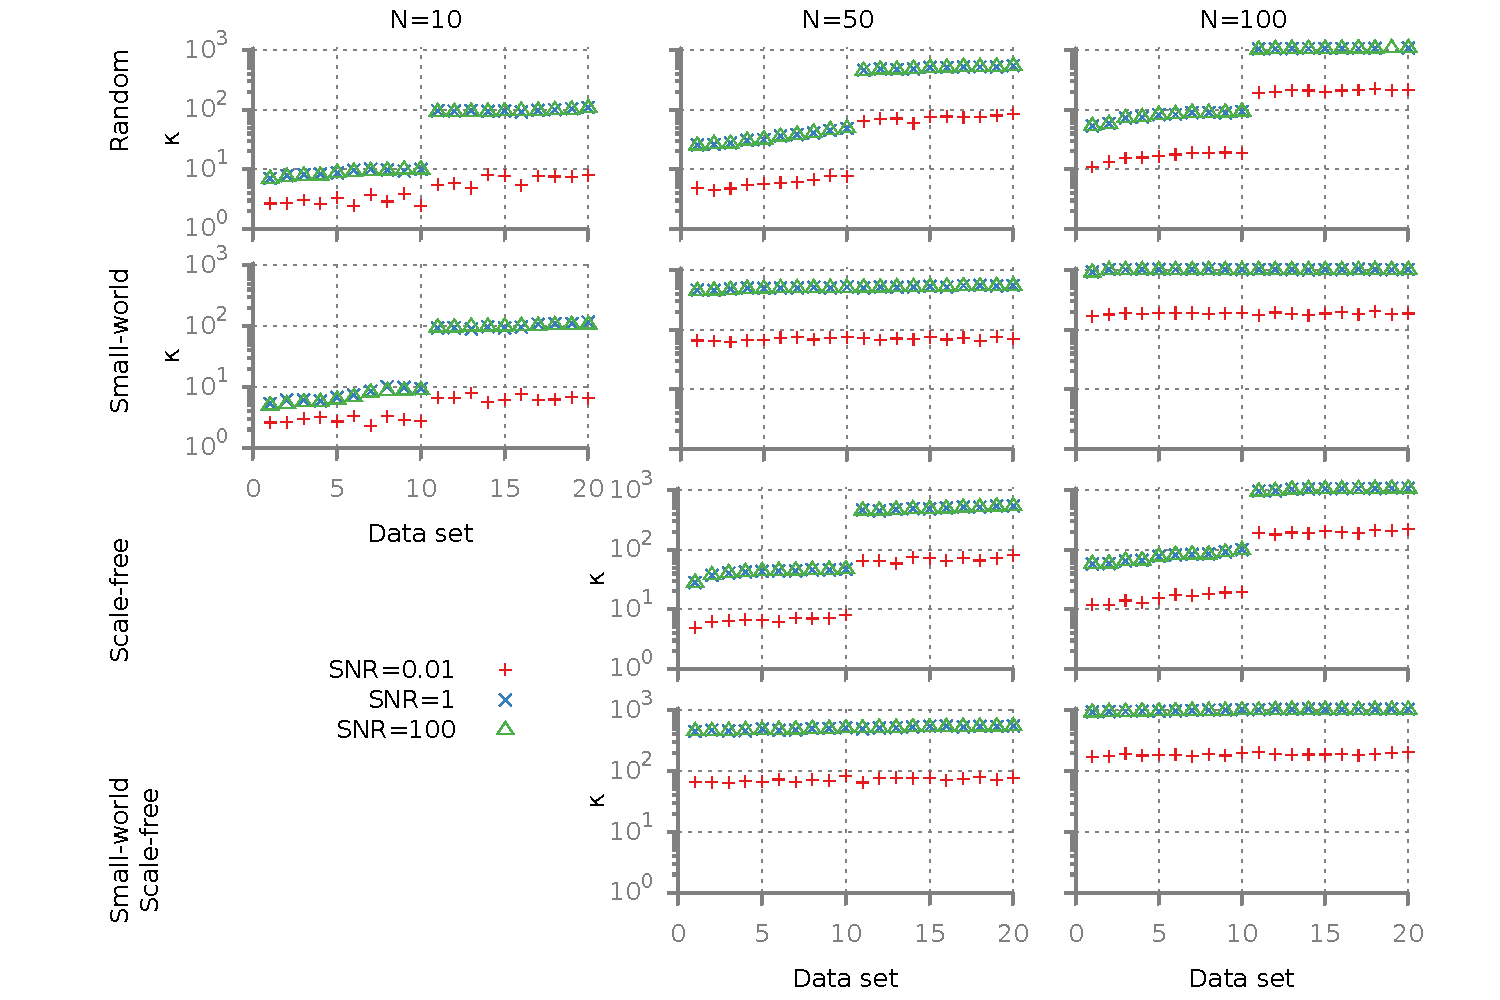
\includegraphics[width=.7\linewidth]{img/data_condition}
\captionsetup{width=.7\textwidth}
\caption{Condition numbers of the response matrices in this benchmark. Three different SNRs were used: $100$, $1$, and $0.01$.  The y-axis shows the condition number $\kappa(\mY)$, and the x-axis shows the number in order of increasing IAA.}
\label{fig:k-data}
\end{figure*}

\subsection{Inference method performance analysis}
\label{sec:analysis-results}
A measure of similarity between the inferred network and the ``true" network used to generate the data is needed to evaluate the performance of inference methods.
% \textcolor{red}{
We here used area under the receiver operating characteristic (AUROC). 
The receiver operating characteristic (ROC) depicts the true-positive rate (TPR), i.e. sensitivity or recall, against the false-positive rate (FPR), i.e. fall-out, as a function of the regularisation parameter for LSCO and Glmnet or the confidence score for RNICO and ARACNe, see the example in Figure \ref{fig:single_performance}.%}

\begin{figure*}[!htb]
\centering
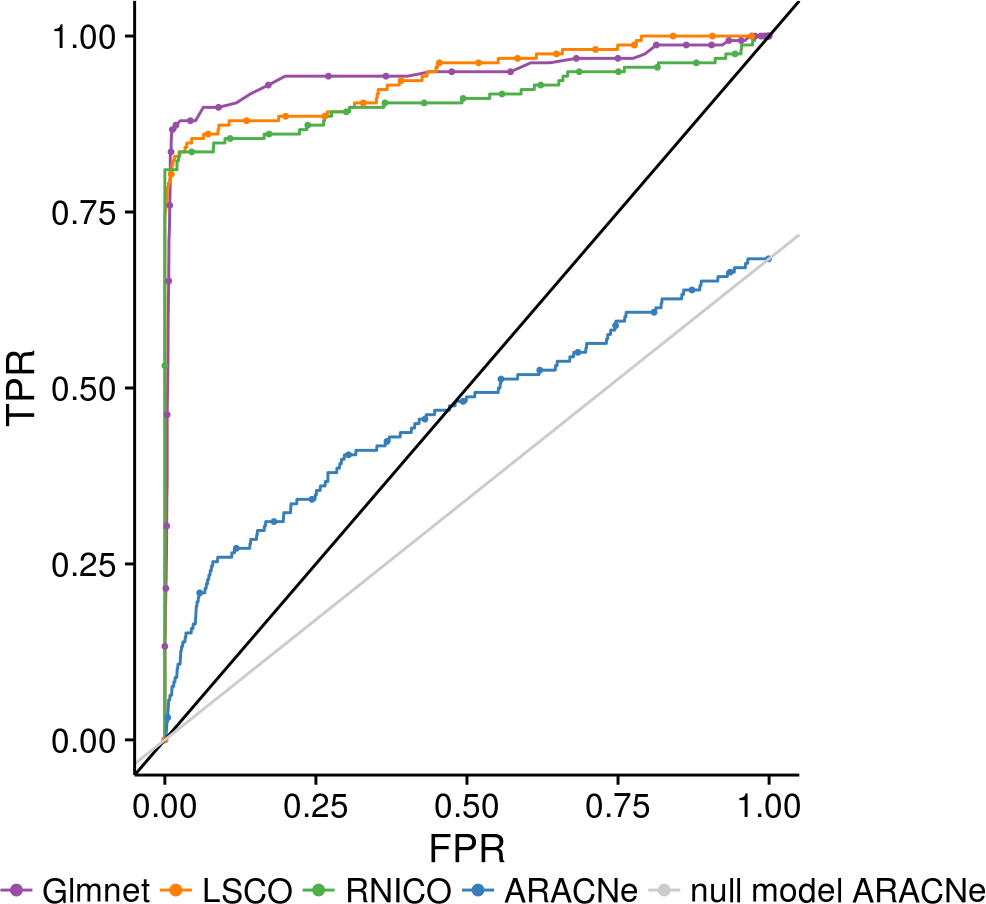
\includegraphics[width=.5\linewidth]{img/ROCcurve.png}
\captionsetup{width=.7\textwidth}
\caption{The ROC curve of four inference methods--Glmnet (\lasso), LSCO, RNICO, and ARACNe--on the Random 50 gene, high IAA, SNR 1 dataset generated by \gs. Note that ARACNe cannot infer self-loops and  therefore has a different null model.}
\label{fig:single_performance}
\end{figure*}

By inferring networks for 100 different values of the regularisation parameter or each confidence score that adds a link we brought the sparsity of the inferred network from an empty network to a full network.
An AUROC of one corresponds to inference of the true network for some regularisation parameter or confidence score with inclusion of all existing links first and then all non-existing ones, while zero corresponds to inclusion of all non-existing links first and then all existing ones such that all networks that can be inferred have the least resemblance to the true network.
% \textcolor{red}{
To compare the four inference methods across the networks and data sets in the benchmark suite, we summarize their AUROC values as bars plots in Figure \ref{fig:performance}. As ARACNe is unable to predict self-loops, we also made a separate benchmark that ignores self-loops entirely (Figure S.3).%}

\begin{figure*}[!htb]
\centering
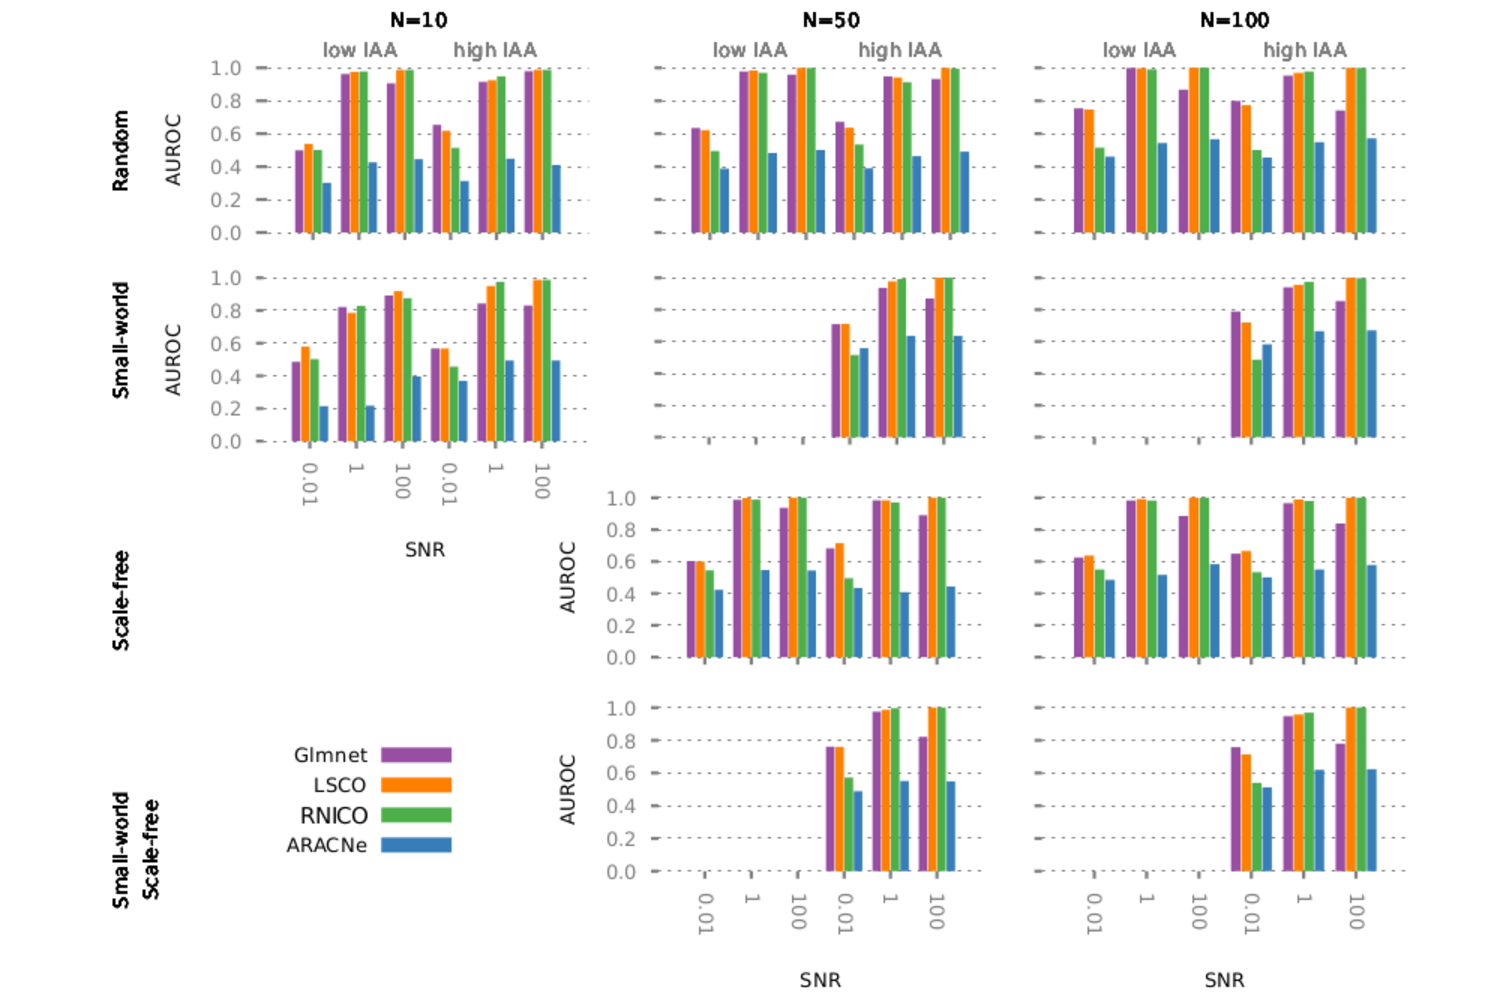
\includegraphics[width=1\linewidth]{img/110117_hasDiag_data_performance}
\captionsetup{width=.7\textwidth}
\caption{Performance of four inference methods -- ARACNe, Glmnet (\lasso), LSCO, and RNICO -- on the benchmark suite  generated by \gs when considering self-loops. The AUROC of an inference method is shown by coloured bars, which are grouped according to IAA degree of the network and SNR of the data (x-axis). The highest and lowest IAA networks were selected among the $20$ networks in each group. Individual ROC curves, MCC plots per sparsity, and density plots per sparsity are available for each condition set in Supplementary Figures, for both considering and not considering self-loops.}
\label{fig:performance}
\end{figure*}

Some major trends can be observed:
\begin{itemize}
\item LSCO and RNICO always give the most accurate networks in cases of SNR 100. The AUROC is almost one and the correct network can in most cases be inferred. RNICO is the preferred method because it can be used to prove the existence of links and provides reliable confidence scores under mild assumptions. To obtain an accurate network using LSCO the correct $\zeta$ value must be selected, while RNICO for a large range of $\zeta$ values will provide accurate networks (Supplementary Figures, MCC panels). However, the correct cut-off to use in RNICO is to set Nordling's confidence score to one, since all links with confidence above one can be proven to exist.

\item Glmnet and ARACNe always fail to infer the correct network when SNR 100, even when LSCO and RNICO succeed, and provide network estimates that are inferior to LSCO and RNICO. This surprising property of Glmnet was previously observed in \cite{Tjarnberg2014}.

\item ARACNe cannot infer self-loops by design, \ie diagonal elements of the interaction matrix. It should therefore be compared to its own null model. Even though it can perform better than random, \ie its null model, in most cases its performance is very poor. ARACNe is clearly outperformed by the other methods in all cases with SNR=1 and 100. For SNR=0.01 it performs similarly to the other methods when not counting self-loops (Figure S.3), but generally close to 0.5 which is the accuracy of random inferences.

\item Glmnet, LSCO, and RNICO have similar AUROC values when SNR= 1, but a good network estimate is given for a narrow range of $\zeta$ values for Glmnet and LSCO, while RNICO yields good estimates for a broad range of values (Supplementary Figures, MCC panels). It is hence easier to obtain a good estimate using RNICO. None of the links can typically be proven to exist using RNICO in this case and the threshold for the confidence score must be selected far below one to get good network estimates.

\item Glmnet is the best method for SNR=0.01 and N=100. In this setting the AUROC values are always below 0.8 however, thus the inferred networks are quite unreliable.

\item In this dataset, changing only the interampatteness gave no clear trend across all methods and property settings.

\item Comparing Figure 3 with Figure S.3, \ie benchmarking with and without considering self-loops, shows that for Glmnet, LSCO, and RNICO this mainly has an effect for SNR=0.01, where the self-loops improve the performance. For N=50 and SNR=0.01, the self-loops alone explain the improvement above random assignment (AUROC=0.5). As expected, ARACNe always scores better when not considering self-loops.

\end{itemize}
\subsection{Benchmark conclusions}
\label{sec:orgheadline8}
The goal of \gs is to provide a common environment for network inference testing and evaluation. We have demonstrated some of its capabilities by generating a benchmark suite of networks and datasets, and used it to analyze the performance of four inference methods.  

It is clear from the benchmarking that mutual information based methods such as ARACNe are generally performing substantially worse than system-optimising methods. This highlights the importance of understanding the system as a whole, which is not achievable by unconnected calculations on the links. ARACNe is further hampered by the fact that it cannot predict self-loops, which are important to bring the system to a stable state, but even if self-loops are ignored its performance is far below the other methods on the two high-SNR settings.
In general, we observed a larger difference in performance in the jump from SNR 0.01 to 1 than from 1 to 100, suggesting a threshold level of noise from which knowledge is recoverable, after which point the noise decrease is less relevant.

Once an algorithm is decided upon, having been vetted against methods of varying strengths and weaknesses, the capability of that choice must be evaluated. Again, our benchmark allowed us to draw the following conclusions:
All methods perform poorly when the SNR is below one because the data simply is not informative enough for network inference.
For high SNRs RNI yields networks that are identical or almost identical to the ``true" network.
\section{Discussion}
\label{discussion}
\gs is a package for GRN inference analysis, for method choice, evaluation and optimization.
It allows the user to control both network and data properties, and contains methods for exploring and analyzing these properties, as well as those of the inference method and its performance.
This opens up new possibilities to understand how these properties affect the performance of inference algorithms.

\gs can create networks with different topological properties that are typical for biological networks.
Given a network, \gs can then simulate expression data that is as informative as typical biological datasets.
However, its unique strength is varying these properties across a wide range of values to gain insights about the limitations and expected performance of a given inference method.
After all, biological data from different sources varies in terms of network and data properties, and the performance of inference methods depend on these properties.
Therefore, when a network inference method is applied to a biological dataset, it is important to make sure that the method has been benchmarked on simulated data with the same properties.
This is not standard practice today, even though it would provide information about the reliability of the inferred network.
%
\gs can also be used to investigate how network properties such as topology and IAA affect data properties.
The nature of the generated data also depends on the experimental design employed for perturbation.
Therefore, \gs supports a range of different experimental design schemes.
For instance, one can control the number of experiments and how many genes are perturbed in each experiment.
This can be of great value when designing wet lab experiments--if a particular design gives optimal results in a benchmark, then it should be the preferred choice when performing real experiments.

It has previously been observed that L$_1$ methods such as Glmnet perform considerably better at low than at high IAA   \citep{Tjarnberg2014}. Such a trend was not clearly observable in this benchmark, probably because the low IAA setting here was not as low as in the previous study.

The \gs package is implemented in \matlab and provides native storage functionality, as well as export options to formats more easily acceptable by other programming languages, including XML and JSON.
\gs fills a gap between theoretical analysis and experimental setup and could be incorporated in many current GRN inference and benchmarking pipelines.

\section{Acknowledgements}
\label{acknowledgements}
This work was partly supported by the Swedish strategic research program eSSENCE, a startup grant by the National Cheng Kung University, and a grant  from the Ministry of science and technology in Taiwan (105-2218-E-006-016-MY2).
%%%END OF MAIN TEXT%%%



%The \balance command can be used to balance the columns on the final page if desired. It should be placed anywhere within the first column of the last page.

%\balance

%If notes are included in your references you can change the title from 'References' to 'Notes and references' using the following command:
%\renewcommand\refname{Notes and references}

%%%REFERENCES%%%
% \bibliography{rsc} %You need to replace "rsc" on this line with the name of your .bib file
% \bibliographystyle{rsc} %the RSC's .bst file
\putbib
\end{bibunit}
\relax 
\providecommand\hyper@newdestlabel[2]{}
\@writefile{toc}{\contentsline {section}{\numberline {S.1}Supplementary Information}{1}{section.24}}
\newlabel{sec:orgheadline24}{{S.1}{1}{Supplementary Information}{section.24}{}}
\@writefile{toc}{\contentsline {subsection}{\numberline {S.1.1}Dependencies of GeneSPIDER\xspace  }{1}{subsection.25}}
\newlabel{sec:dependencies}{{S.1.1}{1}{Dependencies of \gs }{subsection.25}{}}
\@writefile{toc}{\contentsline {subsection}{\numberline {S.1.2}Installation instructions}{1}{subsection.26}}
\newlabel{sec:orgheadline9}{{S.1.2}{1}{Installation instructions}{subsection.26}{}}
\@writefile{toc}{\contentsline {subsection}{\numberline {S.1.3}Notation used for steady-state data}{1}{subsection.27}}
\newlabel{sec:SSnotation}{{S.1.3}{1}{Notation used for steady-state data}{subsection.27}{}}
\newlabel{eq:Linearmap}{{S2}{1}{Notation used for steady-state data}{equation.28}{}}
\newlabel{eqn:MatrixEquationWithErrorsConvertedToRegressors}{{S3}{1}{Notation used for steady-state data}{equation.29}{}}
\newlabel{eqn:MatrixEquationWithErrorsConvertedToRegressorsSystem}{{S3b}{1}{Notation used for steady-state data}{equation.31}{}}
\@writefile{toc}{\contentsline {subsection}{\numberline {S.1.4}Toolboxes}{1}{subsection.32}}
\newlabel{sec:toolboxes}{{S.1.4}{1}{Toolboxes}{subsection.32}{}}
\@writefile{toc}{\contentsline {subsubsection}{\numberline {{S.1.4.1}}Data structure toolbox}{1}{subsubsection.33}}
\newlabel{sec:orgheadline12}{{{S.1.4.1}}{1}{Data structure toolbox}{subsubsection.33}{}}
\newlabel{sec:orgheadline10}{{{S.1.4.1}}{1}{The Network class}{section*.35}{}}
\@writefile{toc}{\contentsline {paragraph}{The Network class}{1}{section*.35}}
\@writefile{lot}{\contentsline {table}{\numberline {S.1}{\ignorespaces  Contents of the \texttt  {datastruct} toolbox.\relax }}{2}{table.caption.34}}
\newlabel{tab:datastruct}{{S.1}{2}{Contents of the \texttt {datastruct} toolbox.\relax }{table.caption.34}{}}
\@writefile{lot}{\contentsline {table}{\numberline {S.2}{\ignorespaces  Methods in the \texttt  {Network} class.\relax }}{2}{table.caption.36}}
\newlabel{tab:network}{{S.2}{2}{Methods in the \texttt {Network} class.\relax }{table.caption.36}{}}
\newlabel{sec:orgheadline11}{{{S.1.4.1}}{2}{The Dataset class}{section*.37}{}}
\@writefile{toc}{\contentsline {paragraph}{The Dataset class}{2}{section*.37}}
\@writefile{lot}{\contentsline {table}{\numberline {S.3}{\ignorespaces  Methods in the \texttt  {Dataset} class.\relax }}{2}{table.caption.38}}
\newlabel{tab:dataset}{{S.3}{2}{Methods in the \texttt {Dataset} class.\relax }{table.caption.38}{}}
\@writefile{toc}{\contentsline {subsubsection}{\numberline {{S.1.4.2}}Analysis toolbox}{2}{subsubsection.39}}
\newlabel{sec:orgheadline15}{{{S.1.4.2}}{2}{Analysis toolbox}{subsubsection.39}{}}
\newlabel{sec:orgheadline13}{{{S.1.4.2}}{2}{The Model class}{section*.41}{}}
\@writefile{toc}{\contentsline {paragraph}{The Model class}{2}{section*.41}}
\newlabel{sec:orgheadline14}{{{S.1.4.2}}{2}{The Data class}{section*.43}{}}
\@writefile{toc}{\contentsline {paragraph}{The Data class}{2}{section*.43}}
\newlabel{sec:compare-models}{{{S.1.4.2}}{2}{The CompareModels class}{section*.45}{}}
\@writefile{lot}{\contentsline {table}{\numberline {S.4}{\ignorespaces  Contents of the \texttt  {analyse} toolbox.\relax }}{3}{table.caption.40}}
\newlabel{tab:analyse}{{S.4}{3}{Contents of the \texttt {analyse} toolbox.\relax }{table.caption.40}{}}
\@writefile{lot}{\contentsline {table}{\numberline {S.5}{\ignorespaces  Methods of \texttt  {Model} class.\relax }}{3}{table.caption.42}}
\newlabel{tab:model}{{S.5}{3}{Methods of \texttt {Model} class.\relax }{table.caption.42}{}}
\@writefile{lot}{\contentsline {table}{\numberline {S.6}{\ignorespaces  Methods of \texttt  {Data} class.\relax }}{3}{table.caption.44}}
\newlabel{tab:data}{{S.6}{3}{Methods of \texttt {Data} class.\relax }{table.caption.44}{}}
\@writefile{toc}{\contentsline {paragraph}{The CompareModels class}{3}{section*.45}}
\@writefile{lot}{\contentsline {table}{\numberline {S.7}{\ignorespaces  System measures\relax }}{3}{table.caption.46}}
\newlabel{tab:sys-measures}{{S.7}{3}{System measures\relax }{table.caption.46}{}}
\@writefile{lot}{\contentsline {table}{\numberline {S.8}{\ignorespaces  Signed topology measures\relax }}{4}{table.caption.47}}
\newlabel{tab:signed-topo-measures}{{S.8}{4}{Signed topology measures\relax }{table.caption.47}{}}
\@writefile{lot}{\contentsline {table}{\numberline {S.9}{\ignorespaces  Correlation measures\relax }}{4}{table.caption.48}}
\newlabel{tab:corr-measures}{{S.9}{4}{Correlation measures\relax }{table.caption.48}{}}
\@writefile{lot}{\contentsline {table}{\numberline {S.10}{\ignorespaces  Graph measures\relax }}{4}{table.caption.49}}
\newlabel{tab:graph-measures}{{S.10}{4}{Graph measures\relax }{table.caption.49}{}}
\@writefile{lot}{\contentsline {table}{\numberline {S.11}{\ignorespaces  Directed graph measures\relax }}{4}{table.caption.50}}
\newlabel{tab:dir-graph-measures}{{S.11}{4}{Directed graph measures\relax }{table.caption.50}{}}
\@writefile{toc}{\contentsline {subsubsection}{\numberline {{S.1.4.3}}Methods toolbox}{4}{subsubsection.51}}
\newlabel{sec:orgheadline16}{{{S.1.4.3}}{4}{Methods toolbox}{subsubsection.51}{}}
\newlabel{eqn:tLSCO}{{S4}{4}{Methods toolbox}{equation.53}{}}
\@writefile{lot}{\contentsline {table}{\numberline {S.12}{\ignorespaces  Method wrappers in GeneSPIDER\xspace  . Each method can be called with a simple unified structure: \texttt  {Methods.<function>(<data>,<parameters>)}.\relax }}{5}{table.caption.52}}
\newlabel{tab:gs-methods}{{S.12}{5}{Method wrappers in \gs . Each method can be called with a simple unified structure: \texttt {Methods.<function>(<data>,<parameters>)}.\relax }{table.caption.52}{}}
\newlabel{eqn:CLS}{{S5}{5}{Methods toolbox}{equation.54}{}}
\newlabel{eqn:CLSObj}{{S5a}{5}{Methods toolbox}{equation.55}{}}
\newlabel{eqn:CLSPredErr}{{S5b}{5}{Methods toolbox}{equation.56}{}}
\newlabel{eqn:CLSR}{{S5c}{5}{Methods toolbox}{equation.57}{}}
\newlabel{eqn:CLSStructure}{{S5d}{5}{Methods toolbox}{equation.58}{}}
\@writefile{toc}{\contentsline {subsubsection}{\numberline {{S.1.4.4}}gsUtilities toolbox}{5}{subsubsection.59}}
\newlabel{sec:orgheadline17}{{{S.1.4.4}}{5}{gsUtilities toolbox}{subsubsection.59}{}}
\@writefile{lot}{\contentsline {table}{\numberline {S.13}{\ignorespaces  Contents of the \texttt  {gsUtilities} toolbox.\relax }}{5}{table.caption.60}}
\newlabel{tab:tool}{{S.13}{5}{Contents of the \texttt {gsUtilities} toolbox.\relax }{table.caption.60}{}}
\@writefile{toc}{\contentsline {subsection}{\numberline {S.1.5}Definitions of data properties}{5}{subsection.61}}
\newlabel{sec:def-data-prop}{{S.1.5}{5}{Definitions of data properties}{subsection.61}{}}
\@writefile{toc}{\contentsline {subsubsection}{\numberline {{S.1.5.1}}Signal to Noise Ratio}{5}{subsubsection.62}}
\newlabel{sec:SNR}{{{S.1.5.1}}{5}{Signal to Noise Ratio}{subsubsection.62}{}}
\newlabel{eq:SNR-phi}{{S6}{5}{Signal to Noise Ratio}{equation.63}{}}
\newlabel{eq:SNR-Phi-true}{{S8}{5}{Signal to Noise Ratio}{equation.65}{}}
\newlabel{eq:SNR-Phi-N}{{S9}{6}{Signal to Noise Ratio}{equation.66}{}}
\newlabel{eq:SNR-def}{{S10}{6}{Signal to Noise Ratio}{equation.67}{}}
\newlabel{eq:SNR-phi-min}{{S10b}{6}{Signal to Noise Ratio}{equation.69}{}}
\@writefile{toc}{\contentsline {subsubsection}{\numberline {{S.1.5.2}}Sample-wise linear dependence}{6}{subsubsection.72}}
\newlabel{sec:orgheadline18}{{{S.1.5.2}}{6}{Sample-wise linear dependence}{subsubsection.72}{}}
\newlabel{eq:eta}{{S11}{6}{Sample-wise linear dependence}{equation.73}{}}
\newlabel{eq:etaexperiments}{{S12}{6}{Sample-wise linear dependence}{equation.74}{}}
\@writefile{toc}{\contentsline {subsection}{\numberline {S.1.6}Generating example data as used in results section}{6}{subsection.75}}
\newlabel{sec:example}{{S.1.6}{6}{Generating example data as used in results section}{subsection.75}{}}
\@writefile{toc}{\contentsline {subsubsection}{\numberline {{S.1.6.1}}Network generation}{6}{subsubsection.76}}
\newlabel{sec:orgheadline19}{{{S.1.6.1}}{6}{Network generation}{subsubsection.76}{}}
\@writefile{lof}{\contentsline {figure}{\numberline {S.1}{\ignorespaces Interampatteness degrees for the networks in the benchmark suite. Each point represents a network, with its IAA degree on the y-axis and its number in order of increasing IAA on the x-axis.\relax }}{7}{figure.caption.77}}
\newlabel{fig:iaa}{{S.1}{7}{Interampatteness degrees for the networks in the benchmark suite. Each point represents a network, with its IAA degree on the y-axis and its number in order of increasing IAA on the x-axis.\relax }{figure.caption.77}{}}
\@writefile{toc}{\contentsline {subsubsection}{\numberline {{S.1.6.2}}Data generation}{7}{subsubsection.79}}
\newlabel{sec:data-generation-example}{{{S.1.6.2}}{7}{Data generation}{subsubsection.79}{}}
\@writefile{lof}{\contentsline {figure}{\numberline {S.2}{\ignorespaces Out-degree distributions for the networks in the benchmark suite. Each distribution is based on 20 individual networks. The y-axis shows the degree frequency, and the x-axis shows the degree.\relax }}{8}{figure.caption.78}}
\newlabel{fig:out-degree}{{S.2}{8}{Out-degree distributions for the networks in the benchmark suite. Each distribution is based on 20 individual networks. The y-axis shows the degree frequency, and the x-axis shows the degree.\relax }{figure.caption.78}{}}
\@writefile{toc}{\contentsline {subsubsection}{\numberline {{S.1.6.3}}Analysis}{9}{subsubsection.80}}
\newlabel{sec:orgheadline23}{{{S.1.6.3}}{9}{Analysis}{subsubsection.80}{}}
\newlabel{sec:orgheadline20}{{{S.1.6.3}}{9}{Network analysis:}{section*.81}{}}
\@writefile{toc}{\contentsline {paragraph}{Network analysis:}{9}{section*.81}}
\newlabel{sec:orgheadline21}{{{S.1.6.3}}{9}{Data analysis:}{section*.82}{}}
\@writefile{toc}{\contentsline {paragraph}{Data analysis:}{9}{section*.82}}
\newlabel{sec:orgheadline22}{{{S.1.6.3}}{10}{Performance evaluation:}{section*.83}{}}
\@writefile{toc}{\contentsline {paragraph}{Performance evaluation:}{10}{section*.83}}
\@writefile{toc}{\contentsline {subsection}{\numberline {S.1.7}Motivations for the design of GeneSPIDER\xspace  }{10}{subsection.84}}
\newlabel{sec:pipeline}{{S.1.7}{10}{Motivations for the design of \gs }{subsection.84}{}}
\@setckpt{supplemental}{
\setcounter{page}{12}
\setcounter{equation}{12}
\setcounter{enumi}{0}
\setcounter{enumii}{0}
\setcounter{enumiii}{0}
\setcounter{enumiv}{0}
\setcounter{footnote}{0}
\setcounter{mpfootnote}{0}
\setcounter{parentequation}{10}
\setcounter{cp@cnt}{1}
\setcounter{cp@tempcnt}{0}
\setcounter{section}{1}
\setcounter{subsection}{7}
\setcounter{subsubsection}{0}
\setcounter{paragraph}{0}
\setcounter{subparagraph}{0}
\setcounter{figure}{2}
\setcounter{table}{13}
\setcounter{NAT@ctr}{25}
\setcounter{Item}{0}
\setcounter{Hfootnote}{0}
\setcounter{bookmark@seq@number}{42}
\setcounter{ContinuedFloat}{0}
\setcounter{section@level}{2}
}

\end{document}
